\documentclass[a4paper,11pt]{article}

\usepackage[utf8]{inputenc}

\usepackage{graphicx}
\usepackage{caption}
\usepackage{subcaption}
\usepackage{float}
\usepackage{amsmath}
\usepackage{array}
\usepackage{multirow}
\usepackage{booktabs}
\usepackage{longtable}
\usepackage[colorlinks=true, linkcolor=blue, urlcolor=blue]{hyperref}

\usepackage{pgfplots}
\pgfplotsset{compat=1.18} 

\usepackage{minted}
\usepackage{pgfplotstable}

\begin{document}

\title{
  \textbf{Breadth-first search}
}
\author{Ying Pei Lin}
\date{Fall 2024}

\maketitle

\subsection*{Introduction}

To traverse a graph by BFS, we start at the root node and explore all the neighbors at the present depth,
before moving on to the nodes at the next depth level. This is done by using a queue to store the nodes
that are to be visited. We take the first node from the queue, visit it, and then add its neighbors to the
queue. We repeat this process until the queue is empty. Following is the pen drawing of the BFS traversal
of a graph.

\begin{figure}[H]
  \centering
  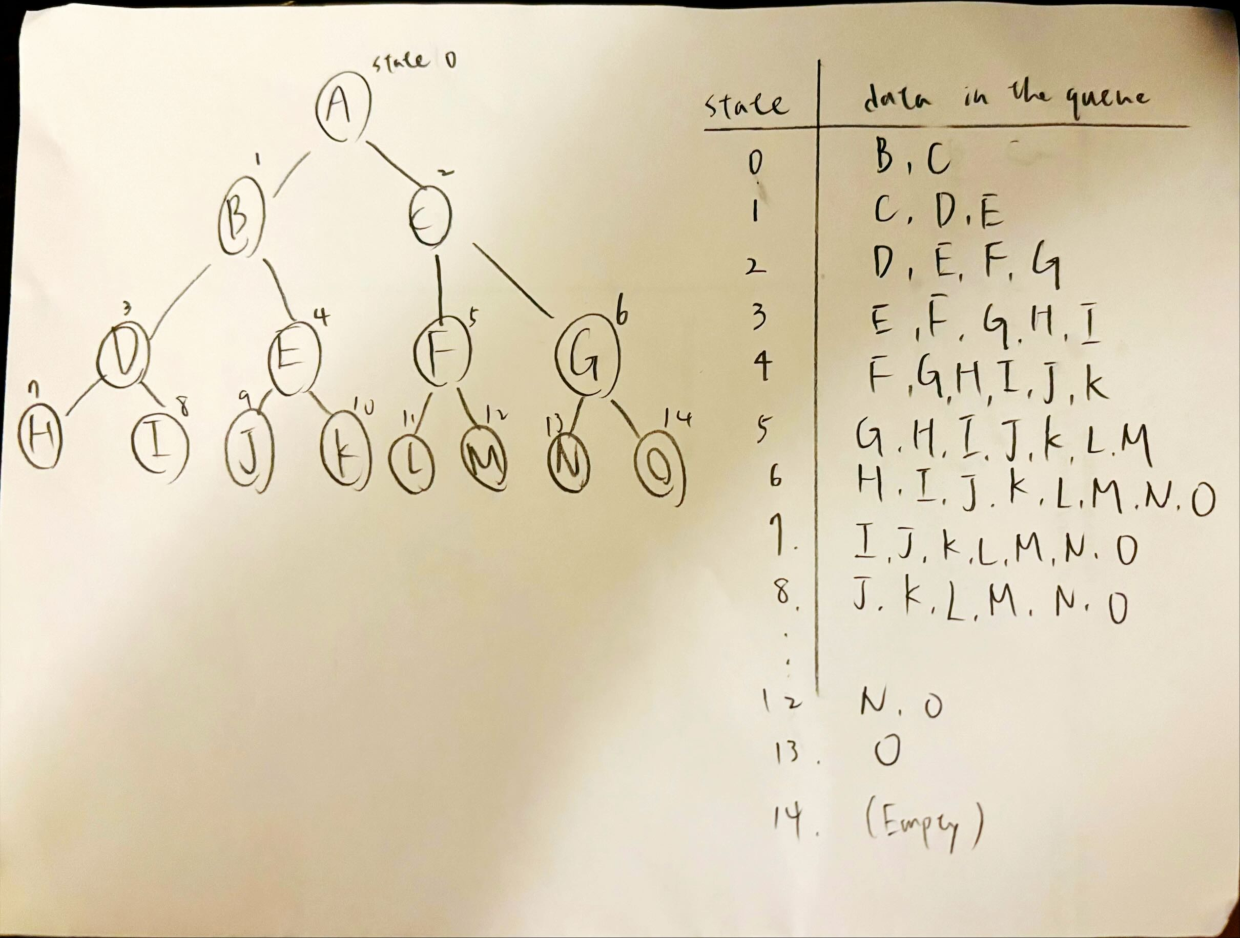
\includegraphics[width=0.5\textwidth]{./draw.pdf}
  \caption{Drawign of BFS traversal of a graph}
\end{figure}

\subsection*{The sequence}

To implement the BFS traversal, we need a tree structure to store the graph, a queue to store the tree
nodes and a sequence to store and get the traversal sequence from the queue. Following are these data
structures.

\begin{minted}{c}
typedef struct TreeNode {
  int value;
  struct TreeNode* left;
  struct TreeNode* right;
} TreeNode;

typedef struct Tree {
  TreeNode* root;
} Tree;

typedef struct QueueNode {
  TreeNode* tree_node;
  struct QueueNode* next;
} QueueNode;

typedef struct Queue {
  QueueNode* front;
  QueueNode* rear;
} Queue;

typedef struct Sequence {
  Queue* queue;
} Sequence;
\end{minted}

The queue structure and its operations will be only used in the sequence structure. We won't use
the queue structure directly. To enqueue a tree node to the queue, we check if the queue is empty
if so, we add the tree node as the first and last node of the queue. Otherwise, we set the new node
as the next node of the last node and update the last node to the new node. The enqueue operation
is shown below.

\begin{minted}{c}
void enqueue(Queue* queue, TreeNode* tree_node) {
  // Create a new queue node
  QueueNode* new_node = (QueueNode*)malloc(sizeof(QueueNode));
  new_node->tree_node = tree_node;
  new_node->next = NULL;

  // Queue is empty
  if (queue->front == NULL && queue->rear == NULL) {
    queue->front = new_node;
    queue->rear = new_node;
    return;
  }

  // Add the new node at the end of queue
  queue->rear->next = new_node;
  queue->rear = new_node;
}
\end{minted}

To dequeue a tree node from the queue, we check if the queue is empty if so, we return NULL. Otherwise,
we get the first node from the queue. If the queue has only one node, then there is no any node left,
so we set the front and rear to NULL. Otherwise, we move the second node to the front. The dequeue
operation is shown below.

\begin{minted}{c}
TreeNode* dequeue(Queue* queue) {
  if(queue->front == NULL && queue->rear == NULL) {
    printf("Queue is empty\n");
    return NULL;
  }

  // Get the first node
  TreeNode* tree_node = queue->front->tree_node;

  // Queue has only one node
  if (queue->front == queue->rear) {
    queue->front = NULL;
    queue->rear = NULL;
  } else {
    // Move the second node to the front
    queue->front = queue->front->next;
  }
  
  return tree_node;
}
\end{minted}

The sequence structure has a queue to store the tree nodes. To initialize the sequence, we create a new
queue and set it to the sequence, and then we add the root node of the tree to the queue. The create
sequence operation is shown below.

\begin{minted}{c}
Sequence* create_sequence(Tree* tree) {
  Sequence* seq = (Sequence*)malloc(sizeof(Sequence));
  seq->queue = create_queue();
  if (tree->root != NULL) {
    enqueue(seq->queue, tree->root);
  }
  return seq;
}
\end{minted}

To get the next tree node from the sequence, we check if the queue is empty if so, we return -1. Otherwise,
we get the first node from the queue by dequeue operation. Then we add the left and right children of the
node to the queue and finally return the value of the node. The next operation is shown below.

\begin{minted}{c}

int next(Sequence* seq) {
  if (seq->queue->front == NULL) {
    return -1;
  }

  // Get the value of the current node
  TreeNode* current = dequeue(seq->queue);

  // Add children to queue
  if (current->left != NULL) {
    enqueue(seq->queue, current->left);
  }
  if (current->right != NULL) {
    enqueue(seq->queue, current->right);
  }

  return current->value;
}
\end{minted}

\subsection*{What happens if we add values to the tree in the break?}

I think the result depends on which parent node we add the new node. Because only in the {\tt next} operation,
we add the children of the current node to the queue. If we add the new node to the visited node, then the
new node won't be added to the queue at any time. If we add new children to nodes that haven't been processed yet, 
they will be included in the traversal sequence at some point.

\subsection*{What could happen if we removed values?}

If the removed node is already in the queue, then pointer in the queue will be invalid and will cause a segmentation
fault. If the removed node is not in the queue or visited, then there is no problem.

\end{document}
